\documentclass[preprint,12pt]{elsarticle}
% Target: Ocean Engineering (Elsevier). elsarticle, numbered references; switch to [review] for double spacing.
\usepackage[utf8]{inputenc}
\usepackage[T1]{fontenc}
\usepackage{amsmath,amssymb}
\usepackage{booktabs,multirow,array}
\usepackage{graphicx}
\usepackage{tikz}
\usetikzlibrary{positioning,arrows.meta,calc}
\usepackage[hidelinks]{hyperref}
\usepackage{xcolor}
\newcommand{\todo}[1]{\textcolor{red}{[TODO: #1]}}
\newcommand{\mapthree}{mAP@0.3}
\journal{Ocean Engineering}
\setlength{\emergencystretch}{3em}

\begin{document}
\begin{frontmatter}
\title{Resolution-preserving tiled detection on SeaClips: a pre-registered study of what transfers to unseen maritime videos, and what does not}

\author[irs]{Anil Kumar Korupoju\corref{cor1}}
\ead{anilkorupoju@outlook.com}
\cortext[cor1]{Corresponding author.}
\affiliation[irs]{organization={\todo{affiliation to confirm}},country={India}}

\begin{abstract}
Camera-based detection of small surface objects is a prerequisite for situational awareness on autonomous and crewed vessels.
We report a pre-registered study on the SeaClips video benchmark, run on a single consumer GPU (12\,GB).
Starting from the benchmark's Deformable-DETR R50 recipe, we replaced the backbone with ConvNeXt-B, trained on a mix of full frames and native-resolution tiles, and detected with a 17-tile scheme.
Every decision gate had a pass rule written before its run; the TEST label file was hash-locked and scored once, after all models were frozen.
Over three seeds, the pre-declared system reached $35.29 \pm 1.09$ TEST \mapthree{}. This is a higher mean than the published TransVOD++ ($31.95 \pm 3.28$) and Deformable-DETR Swin-B ($31.28 \pm 3.72$) baselines, but the differences are not significant under the benchmark's one-tailed Welch test with Bonferroni correction ($p = 0.106$ and $0.098$); the difference from Deformable-DETR R50 ($22.86 \pm 0.91$) is significant ($p = 0.0001$).
A per-class routing of ANIMAL detections to the R50 baseline, chosen on validation data, lowered TEST \mapthree{} in every seed; the unrouted detector, a pre-declared secondary, reached $38.16 \pm 1.41$.
Tiled inference accounted for 13--16 points over each model's own full-frame output, mainly through small objects; SHIP detection remained weak and unstable across seeds.
We report fourteen negative or partial results, five properties of SeaClips that limit what its validation split can show about its test split, and the cost of the approach (about 2\,s per frame). Code and pre-registration records are released; data, predictions and weights are not.

\end{abstract}

\begin{keyword}
maritime object detection \sep autonomous navigation \sep small objects \sep tiled inference \sep Deformable DETR \sep pre-registration \sep negative results \sep SeaClips
\end{keyword}
\end{frontmatter}

\section{Introduction}\label{sec:intro}

Electro-optical cameras are the cheapest sensor on a vessel that can see small, non-cooperative objects: buoys, kayaks, drifting debris, birds on the water and small craft that carry no AIS transponder. Detecting these objects reliably at range is a precondition for collision avoidance on autonomous surface vessels and for decision support on crewed ships. Range makes the task hard: at the distances that matter for manoeuvring, most objects occupy a few pixels of a high-resolution frame, and the conventional practice of resizing a frame to a fixed detector input removes much of that information.

SeaClips \citep{denk2026seaclips} is a recent video benchmark for this problem. It provides 74 annotated videos (47 for training, 9 for validation and 18 for testing) with seven classes, and reports nine baselines evaluated with COCO-style average precision at an intersection-over-union of 0.3 (\mapthree{}), averaged over three seeds. The strongest published results are TransVOD++ with a Swin-B backbone ($31.95 \pm 3.28$) and Deformable DETR with Swin-B ($31.28 \pm 3.72$); Deformable DETR with ResNet-50 reaches $22.86 \pm 0.91$.

Two properties of SeaClips make it hard to know, during development, whether a design choice will help on the test split. First, most objects are very small: at the benchmark's $640 \times 640$ input, the median training box of the ANIMAL class is under 5 pixels across. Second, the validation split represents some test classes poorly or not at all: it contains no LEISURE\_VEHICLE boxes, and all of its ANIMAL boxes come from one video. Our central question is therefore not only whether a detector can score higher on TEST, but which development decisions, made on TRAIN and VAL, transfer to unseen test videos.

We answer it with a pre-registered programme of fifteen gates. For each gate, the hypothesis, the pass rule and the consequence of failure were written down and pinned by file hash before the run. The final system and two pre-declared variants were evaluated once on TEST. The label file had been hash-locked without being parsed, and the evaluation tool refused to run a second time.

The contributions are as follows.
\begin{enumerate}
\item An evaluation of resolution-preserving tile training and 17-tile inference with a ConvNeXt-B Deformable-DETR on SeaClips over three seeds. It is compared with the published baselines and with our own same-pipeline reproduction of the R50 baseline, and reports latency next to accuracy (Section~\ref{sec:results}).
\item A complete account of fourteen negative or partial results. These include a validation-based per-class routing decision that transferred negatively to TEST (Section~\ref{sec:negative}).
\item Five measured properties of SeaClips that bound what its validation split can show about its test split, with recommendations for future evaluations (Section~\ref{sec:dataset}).
\item Released code and pre-registration records. In line with the dataset licence, no images, annotations, predictions or weights are redistributed (Section~\ref{sec:statements}).
\end{enumerate}

We do not claim that the approach outperforms TransVOD++ or Deformable-DETR Swin-B: under the benchmark's own test, the differences in mean are not significant.

\section{Related work}\label{sec:related}

\paragraph{Maritime electro-optical benchmarks}
Prasad et al.\ \citep{prasad2017smd} surveyed electro-optical maritime detection and tracking and introduced the Singapore Maritime Dataset. MODS \citep{bovcon2022mods} targets obstacle detection and segmentation from unmanned surface vehicles. SeaDronesSee \citep{varga2022seadronessee} addresses detection of people in open water from aerial views. SeaClips \citep{denk2026seaclips} provides long, densely annotated surface-level video clips with a test split of 18 unseen videos and reports multi-seed baselines with significance tests. We follow its protocol and compare with its published numbers.

\paragraph{Detectors}
DETR \citep{carion2020detr} formulated detection as set prediction; Deformable DETR \citep{zhu2021deformable} added multi-scale deformable attention, which shortens training and helps small objects. The strongest SeaClips baselines use the Swin Transformer \citep{liu2021swin} as backbone, either per frame or within the video detector TransVOD \citep{zhou2023transvod}. We use ConvNeXt \citep{liu2022convnext} through the timm library \citep{wightman2019timm}, because it fits the memory budget of a 12\,GB GPU at the benchmark resolution.

\paragraph{Small objects and tiled inference}
Slicing a high-resolution image into overlapping tiles, detecting per tile and merging the results is a common way to recover small objects. SAHI \citep{akyon2022sahi} is a widely used example, and Rekavandi et al.\ \citep{rekavandi2022guide} review small-object detection for maritime surveillance. We study tile training and tiled inference under a fixed tile schedule and measure both their accuracy and their cost.

\paragraph{Rare classes}
Repeat-factor sampling \citep{gupta2019lvis} oversamples images that contain rare classes; we test it as one remedy for a collapsing class (Section~\ref{sec:negative}).

\paragraph{Evaluation practice}
Pre-registration separates confirmatory from exploratory analysis \citep{nosek2018prereg}. In machine learning, seed variance can be as large as the differences between methods \citep{bouthillier2021variance}. We combine both: every gate is pre-registered, the final comparison uses three seeds, and we report how decisions made on one seed fared on three.

\section{Dataset and evaluation protocol}\label{sec:protocol}

\subsection{Splits and subsets}
Table~\ref{tab:splits} summarises the splits. All development decisions used TRAIN and VAL only.

\begin{table}[t]
\centering
\caption{SeaClips splits as used in this study. Frame counts were taken from the archive file list.}
\label{tab:splits}
\begin{tabular}{lrrl}
\toprule
Split & Videos & Frames & Use \\
\midrule
TRAIN & 47 & 20{,}310 & training \\
VAL & 9 & 4{,}266 & two 432/426-frame subsets for gates \\
TEST & 18 & 7{,}030 & single final evaluation \\
\bottomrule
\end{tabular}
\end{table}

Running each gate on all VAL frames was too slow for tiled inference on one GPU (about 2\,s per frame), so we defined two disjoint subsets of our own. Within each video, frames are sorted by frame index, and those with index $\equiv 0 \pmod{10}$ (432 frames, the \emph{evaluation} subset) or $\equiv 5 \pmod{10}$ (426 frames, the \emph{selection and replication} subset) are kept. On the R50 baseline, the evaluation subset reproduces full-VAL \mapthree{} to within 0.0004. Because frames are recorded at 30\,frames per second and are strongly correlated, intervals are computed by bootstrap over the nine VAL videos rather than over frames.

\subsection{Metric}
We use pycocotools \citep{lin2014coco} with an IoU threshold of 0.30, at most 100 detections per image, and boxes in original image coordinates, as specified by the benchmark. \mapthree{} is the mean of per-class AP over the classes that have ground truth: seven on TEST and six on VAL, which contains no LEISURE\_VEHICLE. We also report per-class AP, AP for COCO small ($<32^2$\,px), medium and large objects, class-agnostic mAP (mAPca@0.3) and mAP@0.5.

\subsection{Pre-registration and TEST lock}
Each gate was described in a pre-declaration file before it ran: the hypothesis, the data, the arms, a pass rule with numeric thresholds, and the consequence of each outcome. The pre-declaration recorded the SHA-256 of the script that would run. Every long run was preceded by a self-test on synthetic data and a short GPU smoke run that checked resumption, memory and throughput.

Before any final model existed, the TEST label file was hashed without being parsed. The evaluation tool refused any other file, refused to score until every model had been exported, and wrote a lock file after its single run.

\subsection{Statistics}
As in the benchmark paper, we compare the mean of three seeds against each published mean $\pm$ standard deviation ($n=3$) with a one-tailed Welch t-test \citep{welch1947} computed from summary statistics. Degrees of freedom follow Welch--Satterthwaite, and a Bonferroni correction is applied over three comparisons ($\alpha = 0.05/3$). Before TEST was opened we computed that, given the published standard deviation of TransVOD++, a significant difference would require a three-seed mean near 40 \mapthree{}; this fixed the wording of any claim in advance.

\section{Method}\label{sec:method}

Figure~\ref{fig:arch} shows the system. It changes three elements of the benchmark's Deformable-DETR R50 recipe (the backbone, the training crops and the inference scheme) and keeps the rest.

\begin{figure*}[t]
\centering
\resizebox{\textwidth}{!}{% Fig. 1 -- system architecture (TikZ, absolute layout). Compiled inside main.tex.
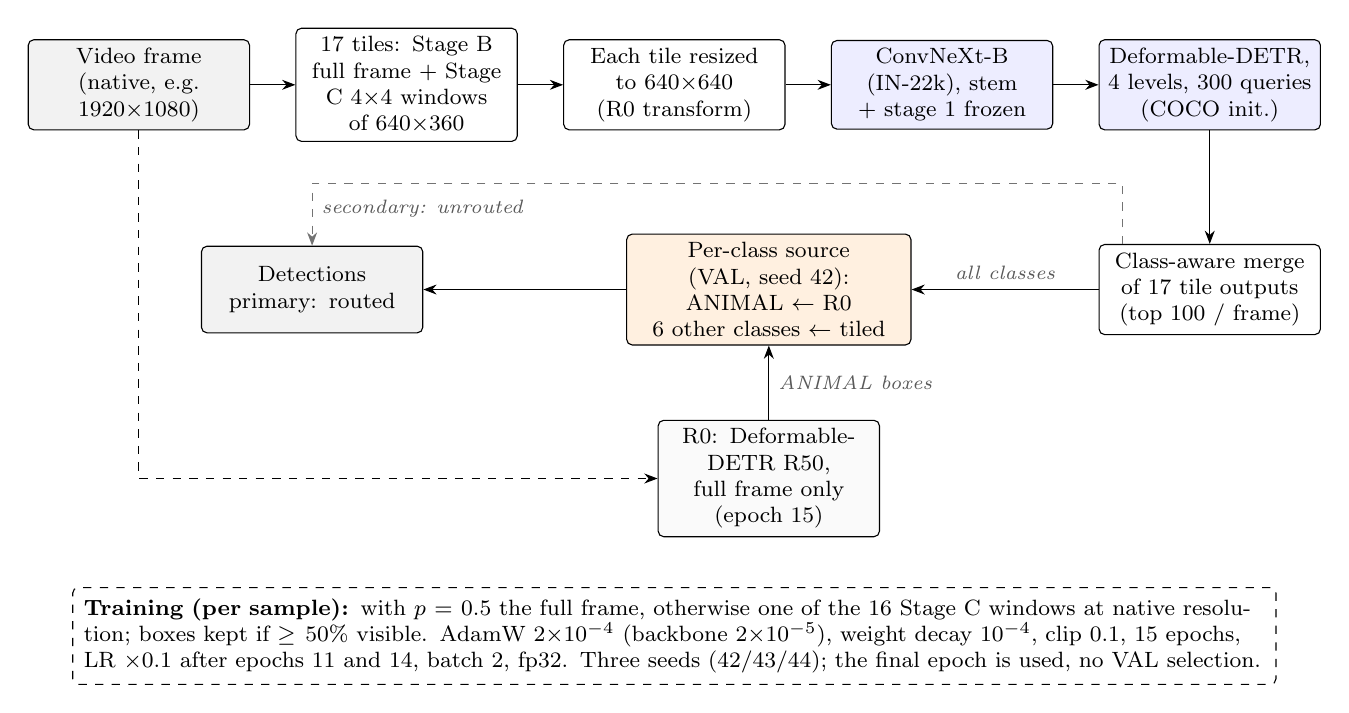
\begin{tikzpicture}[
  font=\footnotesize, >=Stealth,
  box/.style={draw, rounded corners=2pt, align=center, minimum height=11mm, text width=26mm, inner sep=3pt, fill=white},
  data/.style={box, fill=gray!10},
  net/.style={box, fill=blue!7},
  route/.style={box, fill=orange!12, text width=34mm},
  lab/.style={font=\scriptsize\itshape, text=black!65}]
% row 1: tiled detector
\node[data] (frame) at (0,0)    {Video frame\\(native, e.g.\ $1920{\times}1080$)};
\node[box]  (tiles) at (3.4,0)  {17 tiles: Stage B full frame + Stage C $4{\times}4$ windows of $640{\times}360$};
\node[box]  (warp)  at (6.8,0)  {Each tile resized to $640{\times}640$ (R0 transform)};
\node[net]  (bb)    at (10.2,0) {ConvNeXt-B (IN-22k), stem + stage 1 frozen};
\node[net]  (detr)  at (13.6,0) {Deformable-DETR, 4 levels, 300 queries (COCO init.)};
% row 2: merge, routing, output
\node[box]   (merge)  at (13.6,-2.6) {Class-aware merge of 17 tile outputs (top 100 / frame)};
\node[route] (router) at (8.0,-2.6)  {Per-class source (VAL, seed 42):\\ANIMAL $\leftarrow$ R0\\6 other classes $\leftarrow$ tiled};
\node[data]  (out)    at (2.2,-2.6)  {Detections\\primary: routed};
% row 3: R0 branch
\node[box, fill=gray!4] (r0) at (8.0,-5.0) {R0: Deformable-DETR R50, full frame only (epoch 15)};
% arrows
\draw[->] (frame) -- (tiles); \draw[->] (tiles) -- (warp); \draw[->] (warp) -- (bb); \draw[->] (bb) -- (detr);
\draw[->] (detr) -- (merge);
\draw[->] (merge) -- node[lab, above]{all classes} (router);
\draw[->] (router) -- (out);
\draw[->] (r0) -- node[lab, right]{ANIMAL boxes} (router);
\draw[->, dashed] (frame.south) |- (r0.west);
\draw[->, dashed, black!55] (merge.north west) ++(0.3,0) |- (2.2,-1.25) -- node[lab, right, pos=0.4]{secondary: unrouted} (out.north);
% training note
\node[draw, dashed, rounded corners=2pt, align=left, text width=150mm, inner sep=4pt] (train) at (6.8,-7.0) {%
\textbf{Training (per sample):} with $p=0.5$ the full frame, otherwise one of the 16 Stage C windows at native resolution; boxes kept
if $\geq 50\%$ visible. AdamW $2{\times}10^{-4}$ (backbone $2{\times}10^{-5}$), weight decay $10^{-4}$, clip 0.1, 15 epochs,
LR $\times 0.1$ after epochs 11 and 14, batch 2, fp32. Three seeds (42/43/44); the final epoch is used, no VAL selection.};
\end{tikzpicture}
}
\caption{System overview. At inference, each frame is processed as one full-frame tile (Stage~B) and sixteen native-resolution windows (Stage~C); each tile is resized to $640\times640$ and passed through a ConvNeXt-B Deformable-DETR, and the 17 outputs are merged class-aware. In the pre-declared primary system, ANIMAL detections are taken from the full-frame R50 baseline (R0) instead; the unrouted output is a pre-declared secondary. The dashed box summarises training.}
\label{fig:arch}
\end{figure*}

\subsection{Baseline (R0)}
R0 reproduces the benchmark's Deformable-DETR R50 recipe:
\begin{itemize}
\item $640 \times 640$ input without preserving aspect ratio, four feature levels and 300 queries;
\item AdamW with learning rate $2\times10^{-4}$ ($2\times10^{-5}$ for the backbone), weight decay $10^{-4}$ and gradient clipping at 0.1;
\item 15 epochs at batch size 2, with the learning rate divided by 10 after epochs 11 and 14, from a COCO-trained checkpoint.
\end{itemize}
Our reproduction scores 20.72 (epoch 15) and 19.04 (epoch 4, selected on VAL) TEST \mapthree{}, below the published $22.86 \pm 0.91$.

\subsection{Backbone}
The ResNet-50 is replaced by ConvNeXt-B pre-trained on ImageNet-22k (\texttt{convnext\_base.fb\_in22k}, \citep{liu2022convnext,wightman2019timm}). Its four stage outputs feed rebuilt input projections; the stem and first stage are frozen. The transformer, queries and box head are initialised from the COCO checkpoint. A feasibility gate selected ConvNeXt-B as the largest backbone that fits a 12\,GB GPU at the benchmark input with batch size 2. A pilot found bf16 training 0.029 VAL mAP worse than fp32 on R50, so all runs use fp32.

\subsection{Tile training}
Each training sample is, with probability 0.5, the full frame; otherwise it is one of 16 windows of $640\times360$ pixels at native resolution, from a $4\times4$ grid. Boxes are kept if at least 50\% of their area lies inside the window and are clipped to it. The optimiser, learning-rate schedule and number of steps are those of R0.

\subsection{Tiled inference}
At inference, each frame is passed once as a whole (Stage~B) and as the 16 windows (Stage~C), each through R0's $640\times640$ transform. Per-tile detections are mapped to frame coordinates and merged class-aware by a multiscale merge with fixed default constants, no score threshold and the top 100 detections per frame.

\subsection{Per-class routing}
A gate on seed 42 found that the tiled model's ANIMAL head had collapsed on VAL (Section~\ref{sec:negative}). Following a design intent fixed before the TEST evaluation, the source of each class's detections is whichever of the tiled model and the R0 full-frame output has the higher VAL AP30, pooled over both VAL subsets and decided once on seed 42. This routed ANIMAL to R0 (VAL AP 0.116 against 0.0001) and kept the other five VAL classes with the tiled model. LEISURE\_VEHICLE, which has no VAL data, stays with the tiled model. The routed system is the pre-declared primary; the unrouted tiled model is a pre-declared secondary.

\subsection{Seeds and checkpoint}
Seeds 42, 43 and 44 differ only in the random seed, which sets the initialisation of non-transferred layers, the frame order, tile choice, flips and dropout. The final epoch (15) of each seed is used; no checkpoint is selected on VAL.

\section{Experimental programme}\label{sec:programme}

Table~\ref{tab:gates} lists the gates in the order they ran. Two results changed the direction of the study:
\begin{itemize}
\item The first gate (M1) showed that tiled inference with the unchanged R50 model raises recall but adds wrong-class detections, so macro AP does not improve.
\item The backbone pilot (G4 pilot) then showed that a stronger backbone trained on tiles turns the additional recall into AP.
\end{itemize}

\begin{table*}[t]
\centering
\caption{Gates in chronological order (2026-10-27 to 2026-11-04). Each pass rule was fixed before the run. VAL values are macro AP30 on our subsets; $\Delta$ is the paired difference, with a 9-video bootstrap CI where stated.}
\label{tab:gates}
\small
\begin{tabular}{p{1.8cm}p{4.2cm}p{6.3cm}}
\toprule
Gate & Question & Outcome under its pre-declared rule \\
\midrule
M1 / M1.1 & Tiled inference of the frozen R50 & Not met: $\Delta = -0.019$; recall $0.49 \rightarrow 0.68$; merge variants did not help \\
M2 & Tile fine-tune of R50 vs matched control & Not met: $\Delta = +0.014$ (CI $-0.033$ to $0.126$), 4/9 videos; ANIMAL collapsed \\
M2-SL & One class label per query & Closed \\
G1a & Box geometry and horizon as class cues & Failed all three rules \\
G1b-0 & Track-level class vote & Failed: $+0.0128$, 3/6 videos \\
G1c & LEISURE\_VEHICLE census & TRAIN LV is two objects, 0\% small vs 82\% on TEST \\
G2 & Crop class expert with rescoring & Failed: balanced accuracy $-0.018$ \\
G3 & Backbone feasibility (12\,GB) & ConvNeXt-B selected \\
G4 pilot & Tiles vs full frame; backbone; precision & Tiles 0.547 vs 0.461; backbone $+0.155$; fp32 \\
G4 full & ConvNeXt-B + tiles, 15 epochs, vs R50 & Supportive: $+0.136$ (CI $-0.001$ to $0.197$), 7/9 videos; replicated $+0.158$, 6/9 \\
G4b & One-epoch fine-tunes to restore ANIMAL & No arm passed \\
G4c & Anatomy of ANIMAL errors; routing rule & ANIMAL routed to R50 \\
G5 seeds & Seeds 43, 44 (VAL, reported only) & 0.411 and 0.437 vs 0.516 for seed 42 \\
G5 TEST & Three-seed system vs published baselines & Higher mean than all; significant vs R50 only \\
G6 & Rain and sun-flare TEST copies & \todo{pending} \\
\bottomrule
\end{tabular}
\end{table*}

\section{Results on TEST}\label{sec:results}

\subsection{Primary and secondary endpoints}
The pre-declared system scored $35.29 \pm 1.09$ \mapthree{} over three seeds (35.29, 36.39 and 34.21). Table~\ref{tab:primary} gives the pre-registered comparisons. The mean is higher than all published baselines; only the difference from Deformable-DETR R50 is significant after correction.

\begin{table}[t]
\centering
\caption{Primary endpoint: one-tailed Welch test of the three-seed routed system against each published mean $\pm$ SD ($n=3$); Bonferroni $\alpha = 0.0167$.}
\label{tab:primary}
\small
\begin{tabular}{lrrrrc}
\toprule
Comparison & $\Delta$ & $t$ & df & $p$ & Sig. \\
\midrule
TransVOD++ Swin-B ($31.95 \pm 3.28$) & $+3.34$ & 1.68 & 2.44 & 0.106 & no \\
Def.\ DETR Swin-B ($31.28 \pm 3.72$) & $+4.01$ & 1.79 & 2.34 & 0.098 & no \\
Def.\ DETR R50 ($22.86 \pm 0.91$) & $+12.43$ & 15.14 & 3.87 & 0.0001 & yes \\
\bottomrule
\end{tabular}
\end{table}

The unrouted tiled model, a pre-declared secondary, scored $38.16 \pm 1.41$ (36.59, 39.33 and 38.56). Routing ANIMAL to R0 lowered \mapthree{} in every seed, by 1.30, 2.94 and 4.35 points. Exploratory Welch tests of the unrouted model give $p = 0.032$ against TransVOD++ and $p = 0.035$ against Deformable-DETR Swin-B. Both are above the corrected threshold, and neither was a pre-registered hypothesis.

\subsection{Variants, object size and other metrics}
Table~\ref{tab:variants} reports all variants. Each seed's own full-frame (Stage~B) output averages 23.78; tiled inference adds 13--16 points per seed. Small-object AP of the tiled model (31.10) is above every published value; the highest published is 24.98, for RT-DETR. Our R50 reproduction is 2--4 points below the published R50, so our evaluation pipeline does not appear to favour our models. The same-pipeline difference between the routed system and our R0 epoch 15 is $+14.6$.

\begin{table*}[t]
\centering
\caption{TEST results. Ours: mean of three seeds. R0: our R50 reproduction (single run). Paper rows are taken from the SeaClips paper and its supplement (own pipeline).}
\label{tab:variants}
\small
\resizebox{\textwidth}{!}{\begin{tabular}{lrrrrrr}
\toprule
System & \mapthree{} & Small & Medium & Large & mAPca@0.3 & mAP@0.5 \\
\midrule
Ours, routed (primary) & 35.29 & 28.25 & 68.64 & 86.83 & 57.13 & 22.98 \\
Ours, unrouted (secondary) & 38.16 & 31.10 & 68.64 & 86.83 & 57.39 & 26.75 \\
Ours, full frame only & 23.78 & -- & -- & -- & -- & -- \\
R0 epoch 15 (ours) & 20.72 & 16.79 & 49.83 & 52.02 & 39.73 & 10.14 \\
R0 epoch 4, VAL-selected (ours) & 19.04 & 14.85 & 30.30 & 51.76 & 37.23 & 11.36 \\
TransVOD++ Swin-B \citep{denk2026seaclips} & 31.95 & 22.63 & 57.01 & 63.20 & 47.35 & 23.50 \\
Def.\ DETR Swin-B \citep{denk2026seaclips} & 31.28 & 22.93 & 63.72 & 74.06 & 46.64 & 21.70 \\
Def.\ DETR R50 \citep{denk2026seaclips} & 22.86 & 19.22 & 45.44 & 50.08 & 40.63 & 14.87 \\
\bottomrule
\end{tabular}}
\end{table*}

\subsection{Per-class results}
Table~\ref{tab:perclass} gives per-class AP with the range over seeds. The tiled model is higher than every published model on BOAT, SAILING\_VESSEL, LEISURE\_VEHICLE and OBJECT, about equal on MARINE\_MARKER, and lower on SHIP. SHIP also varies most across seeds (17.6 to 42.3). On TEST, the tiled model's ANIMAL AP (39.3 to 60.7) exceeds R0's (30.2): this is why routing lowered TEST mAP, although VAL had indicated the opposite.

\begin{table*}[t]
\centering
\caption{Per-class TEST AP@0.3. Ours: unrouted tiled model, mean and range over three seeds.}
\label{tab:perclass}
\small
\resizebox{\textwidth}{!}{\begin{tabular}{lrrrrrr}
\toprule
Class & Ours & Range & R0 e15 (ours) & TransVOD++ & Swin-B & R50 (paper) \\
\midrule
BOAT & 64.2 & 63.3--64.9 & 40.4 & 48.1 & 51.7 & 37.8 \\
SAILING\_VESSEL & 61.2 & 57.3--65.2 & 38.4 & 36.9 & 45.7 & 35.4 \\
ANIMAL & 50.2 & 39.3--60.7 & 30.2 & 59.8 & 54.2 & 52.8 \\
SHIP & 27.6 & 17.6--42.3 & 6.9 & 48.6 & 31.9 & 9.2 \\
LEISURE\_VEHICLE & 25.0 & 21.1--29.3 & 12.4 & 10.6 & 16.9 & 14.2 \\
OBJECT & 21.9 & 17.9--28.9 & 10.7 & 3.1 & 5.7 & 2.9 \\
MARINE\_MARKER & 17.0 & 13.7--19.6 & 5.9 & 16.6 & 12.8 & 7.9 \\
\bottomrule
\end{tabular}}
\end{table*}

\subsection{Cost}
Export throughput on an RTX 3060, including image decoding, was 1.92--1.97\,s per frame for the 17-tile model and 0.11--0.13\,s per frame for R50 on the full frame (about 2.05--2.10\,s per frame for the routed system). The published models run one $640\times640$ pass per frame. The accuracy gain therefore costs about 17 times the inference compute of a single-pass model of the same size.

\subsection{Robustness to rain and sun flare}\label{sec:robust}
Using the benchmark's corrupted copies of TEST, we evaluate the frozen models once per corruption with the published Albumentations \citep{buslaev2020albumentations} settings. Rain uses \emph{drizzle}, drop width 10, drop length 20 and colour (100,100,100); sun flare uses the physics-based method, flare region of interest (0, 0, 1, 0.3) and source radius 120. Each frame receives a fixed per-frame seed, so every model sees identical corrupted images. \todo{G6 results: table of routed/unrouted/R0 vs paper (R50 5.52 / 18.16; Swin-B 23.71 / 30.11; TransVOD++ 24.47 / 32.64); state the Albumentations version and that the paper's version is unknown.}

\section{Negative and partial results}\label{sec:negative}

Fourteen pre-registered hypotheses failed or passed only partially (Table~\ref{tab:negative}). We report them with their rules so that others need not repeat them. Items 1 to 4 come from a preceding phase of the project, before the gate numbering of Table~\ref{tab:gates}; they used the same R50 baseline and VAL protocol. \todo{expand items 1--4 with their numbers from the project records.}

\begin{table*}[t]
\centering
\caption{Hypotheses that failed or passed only partially.}
\label{tab:negative}
\small
\begin{tabular}{rp{4.0cm}p{2.8cm}p{4.9cm}}
\toprule
\# & Hypothesis & Result & What it shows \\
\midrule
1 & Learned temporal fusion (two-frame, multi-frame, memory) improves R50 & Closed & Gains did not transfer across videos \\
2 & Horizon or vertical-position conditioning helps & Closed & No reliable gain \\
3 & Six auxiliary maritime cues as verifier inputs & Closed & No reliable gain \\
4 & Second stages fitted on R50's TRAIN outputs & Lost 577 VAL true positives & In-sample outputs are unrepresentative: R50 confuses classes on only 0.6\% of TRAIN objects \\
5 & Tiled inference of the frozen R50 (M1) & Not met: $-0.019$ & Recall rose ($0.49 \rightarrow 0.68$); so did wrong-class detections \\
6 & Alternative merge rules (M1.1) & No repair of SAILING\_VESSEL & The loss is classification, not box fusion \\
7 & Tile fine-tune of R50 vs control (M2) & Not met: $+0.014$, 4/9 videos & ANIMAL collapsed and OBJECT halved \\
8 & One class label per query (M2-SL) & Closed & Duplicate labels were not the cause \\
9 & Box geometry and horizon as class cues (G1a) & Failed all rules & The geometry-to-class mapping changes between videos \\
10 & Track-level class vote (G1b-0) & Failed: $+0.0128$, 3/6 videos & Class errors persist along tracks \\
11 & Crop class expert with rescoring (G2) & Failed: $-0.018$ balanced accuracy & Rescoring destroyed per-class ranking (VAL SHIP AP $0.84 \rightarrow 0.10$) \\
12 & ConvNeXt-B + tiles beats R50 on VAL (G4 full) & Supportive only (CI low $-0.001$) & Passed the weaker rule; replicated on the second subset \\
13 & One-epoch fine-tunes restore ANIMAL (G4b) & No arm passed & The collapse was not reversible in one epoch; repeat-factor sampling raised false positives \\
14 & VAL-chosen per-class routing helps on TEST (G5 primary) & $-1.3$ to $-4.4$ per seed & A one-video validation class does not represent TEST \\
\bottomrule
\end{tabular}
\end{table*}

\paragraph{The ANIMAL collapse}
On VAL, all three ConvNeXt-B seeds had ANIMAL AP near zero. In seed 42, the tiled model found 4 of the 52 pooled VAL ANIMAL boxes and R50 found 6, so recall was similar. The difference was precision: the tiled model emitted 2{,}897 ANIMAL detections with score $\geq 0.05$ that matched no ANIMAL box. Of these, 833 lay on marine markers and 1{,}750 on background, and 341 scored above the best true detection. Most (2{,}258) were also produced by the full-frame tile, so they were learned, not an artefact of tiling. None of three one-epoch remedies reversed this: further tile training, full frames only, and repeat-factor sampling with ANIMAL-aware window choice \citep{gupta2019lvis}. On TEST, however, the same models reached 39--61 ANIMAL AP; the VAL video was not representative (Section~\ref{sec:dataset}).

\paragraph{Decisions taken on one seed}
G4, G4b and G4c were decided on seed 42 alone. On VAL, seeds 43 and 44 later scored 0.105 and 0.079 lower than seed 42 in tiled macro AP30. The spread concentrated in vessel classes: SHIP 0.58--0.78, BOAT 0.31--0.55 and SAILING\_VESSEL 0.72--0.95, while MARINE\_MARKER stayed at 0.48--0.52. On TEST the ordering reversed: seed 42 was the lowest of the three unrouted models.

\paragraph{Process faults}
Two engineering faults were caught by the mandatory smoke runs before any long job.
\begin{itemize}
\item A resume check assumed bit-exact GPU training, but the deformable-attention sampling kernels are not deterministic. The check was replaced by a bound relative to fresh-run noise.
\item An import-order dependency in the Windows environment.
\end{itemize}

\section{Properties of SeaClips that limit validation}\label{sec:dataset}

We measured five properties of SeaClips that bound what its validation split can say about its test split. They were measured from annotations, from the public counts in the benchmark supplement, or from model outputs on TRAIN and VAL.

\paragraph{1. Two TEST classes cannot be validated as they appear on TEST}
LEISURE\_VEHICLE has no VAL boxes. Its 600 TRAIN boxes show two physical objects in two videos from one camera in sunny, calm conditions, and none is COCO-small; on TEST, 82\% of the class (9{,}912 of 12{,}115 boxes) is small. All 253 VAL ANIMAL boxes are in one video (median $\sqrt{\text{area}}$ 9.4\,px; 22\% below 8\,px). The ANIMAL routing decision taken on that video reversed on TEST.

\paragraph{2. Validation level does not predict test level}
R50 scores 0.42 on VAL and 19--21 on TEST. Across our three seeds, the VAL ranking (0.516, 0.437, 0.411 for seeds 42, 44, 43) was the reverse of the unrouted TEST ranking (36.59, 38.56, 39.33). Single-seed VAL comparisons are therefore weak evidence for TEST.

\paragraph{3. VAL scores swing within a run}
At the full learning rate, VAL mAP on our selection subset moved by about $\pm 0.06$ between epochs while the training loss fell smoothly. It settled to within about 0.02 after the first learning-rate decay. Selecting checkpoints on VAL is correspondingly noisy.

\paragraph{4. Many objects are a few pixels wide at the standard input}
After the benchmark's $640 \times 640$ resize, the median TRAIN ANIMAL box is 4.7\,px across, and the 10th percentile is 2.4\,px. A third of TRAIN ANIMAL boxes are below 8\,px even at native resolution. This favours native-resolution inference. It may also teach a shortcut ("a few-pixel blob is ANIMAL"); our models labelled buoys and clutter as ANIMAL on VAL.

\paragraph{5. The dominant error is classification, not localisation}
On VAL, an oracle analysis of the tile-trained R50 (0.380 macro AP30) bounds the gain from removing each error type. Removing background false positives gives 0.402; also removing part-of-object detections, 0.414; also removing wrong-class detections, 0.583. On TEST, seed-to-seed variance concentrated in vessel types (SHIP 17.6--42.3), while MARINE\_MARKER was stable.

\paragraph{Recommendations}
\begin{itemize}
\item Report several seeds, and bootstrap intervals over videos for VAL.
\item Do not select per-class components on VAL classes drawn from a single video.
\item Where TRAIN allows, hold out TRAIN videos for classes that VAL does not represent.
\item Report latency next to accuracy for native-resolution methods.
\end{itemize}

\section{Discussion}\label{sec:discussion}

\subsection{Lessons}
\begin{enumerate}
\item \textbf{Pre-declare secondaries, not only primaries.} The unrouted detector was declared as a secondary endpoint before TEST, so its result (38.16) can be reported. Equally, it cannot replace the primary after the fact.
\item \textbf{Check that a validation class represents TEST before choosing per-class components on it.} A single VAL video decided the ANIMAL routing, and TEST disagreed by 9 to 31 AP per seed.
\item \textbf{Run several seeds before architectural decisions, not only at the end.} One seed led four gates; it was the most favourable seed on VAL and the least favourable on TEST.
\item \textbf{Compute the significance threshold before TEST.} With the published standard deviations and $n = 3$, a significant difference from TransVOD++ needed a mean near 40. Knowing this beforehand fixed the claim language.
\item \textbf{Prove long runs before starting them.} Synthetic self-tests and GPU smoke runs caught every pipeline fault we met before a multi-hour job started.
\end{enumerate}

\subsection{Limitations and threats to validity}
\begin{itemize}
\item \textbf{Statistical power.} Three seeds, compared against published summary statistics rather than per-seed values, give a Welch test with low power.
\item \textbf{Two pipelines.} The baselines were produced by the benchmark authors, and our numbers by our pycocotools-based evaluator. The protocol matches as far as it is documented: IoU 0.3, seven classes, original-image boxes and all TEST frames. Our R50 reproduction is 2--4 points below the published R50, so the evaluator does not appear to favour our models; the same-pipeline difference is the more conservative comparison.
\item \textbf{Shared routing source.} The routed system uses one R50 model for all seeds, so its standard deviation understates the variance of the full system.
\item \textbf{Reuse of VAL.} VAL-based gates reused the same nine videos many times; TEST is the only independent check.
\item \textbf{Cost.} Tiled inference costs 17 forward passes per frame, about 2\,s on an RTX 3060. Real-time use would require a cheaper tiling or a lighter backbone.
\item \textbf{Robustness.} The robustness results depend on the Albumentations version, and the version used by the benchmark authors is not stated.
\end{itemize}

\section{Conclusion}\label{sec:conclusion}

On SeaClips TEST, the pre-declared system reached $35.29 \pm 1.09$ \mapthree{} over three seeds, and its unrouted variant $38.16 \pm 1.41$. Both means are higher than the published baselines; under the benchmark's test, only the comparison with Deformable-DETR R50 is significant. Resolution-preserving tile training and tiled inference produced most of the difference, especially for small objects. Classifying vessel types across unseen videos remains the open problem. A validation-based routing decision transferred negatively, which illustrates the limits of SeaClips' validation split documented here.

Future work:
\begin{itemize}
\item cheaper tilings, measured as an accuracy--latency curve;
\item vessel-type classification across videos;
\item validation designs that hold out TRAIN videos for classes the validation split cannot represent.
\end{itemize}

\section*{Code and data availability}\label{sec:statements}
Code, pre-registration records with script hashes, and aggregate results are available at \url{https://github.com/<user>/marivision} \todo{final URL; anonymised copy if the review is double-blind}. SeaClips images, annotations, per-frame predictions and trained weights are not redistributed, in line with the dataset licence. Reproduction requires obtaining SeaClips from its maintainers.

\section*{Declaration of generative AI use}
\todo{Write to the journal's policy: AI assistance (Claude, Anthropic) was used for code development, analysis tooling and drafting; the author reviewed and takes responsibility for all content.}

\section*{CRediT authorship contribution statement}
\textbf{Anil Kumar Korupoju:} Conceptualization, Methodology, Investigation, Software, Validation, Writing -- original draft, Writing -- review \& editing. \todo{co-authors}

\section*{Declaration of competing interest}
\todo{The author declares no competing interests.}

\section*{Acknowledgements}
We thank the SeaClips authors for releasing the benchmark. \todo{funding}


\bibliographystyle{elsarticle-num}
\bibliography{refs}
\end{document}
